%% bare_conf.tex
%% V1.4
%% 2012/12/27
%% by Michael Shell
%% See:
%% http://www.michaelshell.org/
%% for current contact information.
%%
%% This is a skeleton file demonstrating the use of IEEEtran.cls
%% (requires IEEEtran.cls version 1.8 or later) with an IEEE conference paper.
%%
%% Support sites:
%% http://www.michaelshell.org/tex/ieeetran/
%% http://www.ctan.org/tex-archive/macros/latex/contrib/IEEEtran/
%% and
%% http://www.ieee.org/

%%*************************************************************************
%% Legal Notice:
%% This code is offered as-is without any warranty either expressed or
%% implied; without even the implied warranty of MERCHANTABILITY or
%% FITNESS FOR A PARTICULAR PURPOSE!
%% User assumes all risk.
%% In no event shall IEEE or any contributor to this code be liable for
%% any damages or losses, including, but not limited to, incidental,
%% consequential, or any other damages, resulting from the use or misuse
%% of any information contained here.
%%
%% All comments are the opinions of their respective authors and are not
%% necessarily endorsed by the IEEE.
%%
%% This work is distributed under the LaTeX Project Public License (LPPL)
%% ( http://www.latex-project.org/ ) version 1.3, and may be freely used,
%% distributed and modified. A copy of the LPPL, version 1.3, is included
%% in the base LaTeX documentation of all distributions of LaTeX released
%% 2003/12/01 or later.
%% Retain all contribution notices and credits.
%% ** Modified files should be clearly indicated as such, including  **
%% ** renaming them and changing author support contact information. **
%%
%% File list of work: IEEEtran.cls, IEEEtran_HOWTO.pdf, bare_adv.tex,
%%                    bare_conf.tex, bare_jrnl.tex, bare_jrnl_compsoc.tex,
%%                    bare_jrnl_transmag.tex
%%*************************************************************************

% *** Authors should verify (and, if needed, correct) their LaTeX system  ***
% *** with the testflow diagnostic prior to trusting their LaTeX platform ***
% *** with production work. IEEE's font choices can trigger bugs that do  ***
% *** not appear when using other class files.                            ***
% The testflow support page is at:
% http://www.michaelshell.org/tex/testflow/



% Note that the a4paper option is mainly intended so that authors in
% countries using A4 can easily print to A4 and see how their papers will
% look in print - the typesetting of the document will not typically be
% affected with changes in paper size (but the bottom and side margins will).
% Use the testflow package mentioned above to verify correct handling of
% both paper sizes by the user's LaTeX system.
%
% Also note that the "draftcls" or "draftclsnofoot", not "draft", option
% should be used if it is desired that the figures are to be displayed in
% draft mode.
%
\documentclass[conference]{IEEEtran}
% Add the compsoc option for Computer Society conferences.
%
% If IEEEtran.cls has not been installed into the LaTeX system files,
% manually specify the path to it like:
% \documentclass[conference]{../sty/IEEEtran}





% Some very useful LaTeX packages include:
% (uncomment the ones you want to load)


% *** MISC UTILITY PACKAGES ***
%
%\usepackage{ifpdf}
% Heiko Oberdiek's ifpdf.sty is very useful if you need conditional
% compilation based on whether the output is pdf or dvi.
% usage:
% \ifpdf
%   % pdf code
% \else
%   % dvi code
% \fi
% The latest version of ifpdf.sty can be obtained from:
% http://www.ctan.org/tex-archive/macros/latex/contrib/oberdiek/
% Also, note that IEEEtran.cls V1.7 and later provides a builtin
% \ifCLASSINFOpdf conditional that works the same way.
% When switching from latex to pdflatex and vice-versa, the compiler may
% have to be run twice to clear warning/error messages.


% *** CITATION PACKAGES ***
%
\usepackage{cite}
% cite.sty was written by Donald Arseneau
% V1.6 and later of IEEEtran pre-defines the format of the cite.sty package
% \cite{} output to follow that of IEEE. Loading the cite package will
% result in citation numbers being automatically sorted and properly
% "compressed/ranged". e.g., [1], [9], [2], [7], [5], [6] without using
% cite.sty will become [1], [2], [5]--[7], [9] using cite.sty. cite.sty's
% \cite will automatically add leading space, if needed. Use cite.sty's
% noadjust option (cite.sty V3.8 and later) if you want to turn this off
% such as if a citation ever needs to be enclosed in parenthesis.
% cite.sty is already installed on most LaTeX systems. Be sure and use
% version 4.0 (2003-05-27) and later if using hyperref.sty. cite.sty does
% not currently provide for hyperlinked citations.
% The latest version can be obtained at:
% http://www.ctan.org/tex-archive/macros/latex/contrib/cite/
% The documentation is contained in the cite.sty file itself.



% *** GRAPHICS RELATED PACKAGES ***
%
\ifCLASSINFOpdf
  \usepackage[pdftex]{graphicx}
  % declare the path(s) where your graphic files are
  % \graphicspath{{../pdf/}{../jpeg/}}
  % and their extensions so you won't have to specify these with
  % every instance of \includegraphics
  \DeclareGraphicsExtensions{.pdf,.jpeg,.png}
\else
  % or other class option (dvipsone, dvipdf, if not using dvips). graphicx
  % will default to the driver specified in the system graphics.cfg if no
  % driver is specified.
  \usepackage[dvips]{graphicx}
  % declare the path(s) where your graphic files are
  % \graphicspath{{../eps/}}
  % and their extensions so you won't have to specify these with
  % every instance of \includegraphics
  \DeclareGraphicsExtensions{.eps}
\fi
% graphicx was written by David Carlisle and Sebastian Rahtz. It is
% required if you want graphics, photos, etc. graphicx.sty is already
% installed on most LaTeX systems. The latest version and documentation
% can be obtained at:
% http://www.ctan.org/tex-archive/macros/latex/required/graphics/
% Another good source of documentation is "Using Imported Graphics in
% LaTeX2e" by Keith Reckdahl which can be found at:
% http://www.ctan.org/tex-archive/info/epslatex/
%
% latex, and pdflatex in dvi mode, support graphics in encapsulated
% postscript (.eps) format. pdflatex in pdf mode supports graphics
% in .pdf, .jpeg, .png and .mps (metapost) formats. Users should ensure
% that all non-photo figures use a vector format (.eps, .pdf, .mps) and
% not a bitmapped formats (.jpeg, .png). IEEE frowns on bitmapped formats
% which can result in "jaggedy"/blurry rendering of lines and letters as
% well as large increases in file sizes.
%
% You can find documentation about the pdfTeX application at:
% http://www.tug.org/applications/pdftex
\usepackage{lipsum}


% *** MATH PACKAGES ***
%
\usepackage[cmex10]{amsmath}
% A popular package from the American Mathematical Society that provides
% many useful and powerful commands for dealing with mathematics. If using
% it, be sure to load this package with the cmex10 option to ensure that
% only type 1 fonts will utilized at all point sizes. Without this option,
% it is possible that some math symbols, particularly those within
% footnotes, will be rendered in bitmap form which will result in a
% document that can not be IEEE Xplore compliant!
%
% Also, note that the amsmath package sets \interdisplaylinepenalty to 10000
% thus preventing page breaks from occurring within multiline equations. Use:
%\interdisplaylinepenalty=2500
% after loading amsmath to restore such page breaks as IEEEtran.cls normally
% does. amsmath.sty is already installed on most LaTeX systems. The latest
% version and documentation can be obtained at:
% http://www.ctan.org/tex-archive/macros/latex/required/amslatex/math/





% *** SPECIALIZED LIST PACKAGES ***
%
%\usepackage{algorithmic}
% algorithmic.sty was written by Peter Williams and Rogerio Brito.
% This package provides an algorithmic environment fo describing algorithms.
% You can use the algorithmic environment in-text or within a figure
% environment to provide for a floating algorithm. Do NOT use the algorithm
% floating environment provided by algorithm.sty (by the same authors) or
% algorithm2e.sty (by Christophe Fiorio) as IEEE does not use dedicated
% algorithm float types and packages that provide these will not provide
% correct IEEE style captions. The latest version and documentation of
% algorithmic.sty can be obtained at:
% http://www.ctan.org/tex-archive/macros/latex/contrib/algorithms/
% There is also a support site at:
% http://algorithms.berlios.de/index.html
% Also of interest may be the (relatively newer and more customizable)
% algorithmicx.sty package by Szasz Janos:
% http://www.ctan.org/tex-archive/macros/latex/contrib/algorithmicx/




% *** ALIGNMENT PACKAGES ***
%
%\usepackage{array}
% Frank Mittelbach's and David Carlisle's array.sty patches and improves
% the standard LaTeX2e array and tabular environments to provide better
% appearance and additional user controls. As the default LaTeX2e table
% generation code is lacking to the point of almost being broken with
% respect to the quality of the end results, all users are strongly
% advised to use an enhanced (at the very least that provided by array.sty)
% set of table tools. array.sty is already installed on most systems. The
% latest version and documentation can be obtained at:
% http://www.ctan.org/tex-archive/macros/latex/required/tools/


% IEEEtran contains the IEEEeqnarray family of commands that can be used to
% generate multiline equations as well as matrices, tables, etc., of high
% quality.


% *** SUBFIGURE PACKAGES ***
\ifCLASSOPTIONcompsoc
  \usepackage[caption=false,font=normalsize,labelfont=sf,textfont=sf]{subfig}
\else
  \usepackage[caption=false,font=footnotesize]{subfig}
\fi
% subfig.sty, written by Steven Douglas Cochran, is the modern replacement
% for subfigure.sty, the latter of which is no longer maintained and is
% incompatible with some LaTeX packages including fixltx2e. However,
% subfig.sty requires and automatically loads Axel Sommerfeldt's caption.sty
% which will override IEEEtran.cls' handling of captions and this will result
% in non-IEEE style figure/table captions. To prevent this problem, be sure
% and invoke subfig.sty's "caption=false" package option (available since
% subfig.sty version 1.3, 2005/06/28) as this is will preserve IEEEtran.cls
% handling of captions.
% Note that the Computer Society format requires a larger sans serif font
% than the serif footnote size font used in traditional IEEE formatting
% and thus the need to invoke different subfig.sty package options depending
% on whether compsoc mode has been enabled.
%
% The latest version and documentation of subfig.sty can be obtained at:
% http://www.ctan.org/tex-archive/macros/latex/contrib/subfig/
\usepackage{multirow,siunitx}



% *** FLOAT PACKAGES ***
%
\usepackage{fixltx2e}
% fixltx2e, the successor to the earlier fix2col.sty, was written by
% Frank Mittelbach and David Carlisle. This package corrects a few problems
% in the LaTeX2e kernel, the most notable of which is that in current
% LaTeX2e releases, the ordering of single and double column floats is not
% guaranteed to be preserved. Thus, an unpatched LaTeX2e can allow a
% single column figure to be placed prior to an earlier double column
% figure. The latest version and documentation can be found at:
% http://www.ctan.org/tex-archive/macros/latex/base/


%\usepackage{stfloats}
% stfloats.sty was written by Sigitas Tolusis. This package gives LaTeX2e
% the ability to do double column floats at the bottom of the page as well
% as the top. (e.g., "\begin{figure*}[!b]" is not normally possible in
% LaTeX2e). It also provides a command:
%\fnbelowfloat
% to enable the placement of footnotes below bottom floats (the standard
% LaTeX2e kernel puts them above bottom floats). This is an invasive package
% which rewrites many portions of the LaTeX2e float routines. It may not work
% with other packages that modify the LaTeX2e float routines. The latest
% version and documentation can be obtained at:
% http://www.ctan.org/tex-archive/macros/latex/contrib/sttools/
% Do not use the stfloats baselinefloat ability as IEEE does not allow
% \baselineskip to stretch. Authors submitting work to the IEEE should note
% that IEEE rarely uses double column equations and that authors should try
% to avoid such use. Do not be tempted to use the cuted.sty or midfloat.sty
% packages (also by Sigitas Tolusis) as IEEE does not format its papers in
% such ways.
% Do not attempt to use stfloats with fixltx2e as they are incompatible.
% Instead, use Morten Hogholm'a dblfloatfix which combines the features
% of both fixltx2e and stfloats:
%
% \usepackage{dblfloatfix}
% The latest version can be found at:
% http://www.ctan.org/tex-archive/macros/latex/contrib/dblfloatfix/




% *** PDF, URL AND HYPERLINK PACKAGES ***
%
%\usepackage{url}
% url.sty was written by Donald Arseneau. It provides better support for
% handling and breaking URLs. url.sty is already installed on most LaTeX
% systems. The latest version and documentation can be obtained at:
% http://www.ctan.org/tex-archive/macros/latex/contrib/url/
% Basically, \url{my_url_here}.


%***CHEMISTRY PACKAGES***%
\usepackage[version=4]{mhchem}

% *** Do not adjust lengths that control margins, column widths, etc. ***
% *** Do not use packages that alter fonts (such as pslatex).         ***
% There should be no need to do such things with IEEEtran.c\hlinels V1.6 and later.
% (Unless specifically asked to do so by the journal or conference you plan
% to submit to, of course. )


% correct bad hyphenation here
\hyphenation{op-tical net-works semi-conduc-tor}


\begin{document}
%
% paper title
% can use linebreaks \\ within to get better formatting as desired
% Do not put math or special symbols in the title.
\title{Using Deep Learning and EMG to recognize non-audible speech}


% author names and affiliations
% use a multiple column layout for up to three different
% affiliations
\author{\IEEEauthorblockN{Rommel T. Fernandes}
\IEEEauthorblockA{\textit{Seaver College of Science and Engineering}\\
\textit{Loyola Marymount University}\\
\textit{Los Angeles, CA, USA}\\
\textit{Email: rferna16@lion.lmu.edu}}
}

% conference papers do not typically use \thanks and this command
% is locked out in conference mode. If really needed, such as for
% the acknowledgment of grants, issue a \IEEEoverridecommandlockouts
% after \documentclass

% for over three affiliations, or if they all won't fit within the width
% of the page, use this alternative format:
%
%\author{\IEEEauthorblockN{Michael Shell\IEEEauthorrefmark{1},
%Homer Simpson\IEEEauthorrefmark{2},
%James Kirk\IEEEauthorrefmark{3},
%Montgomery Scott\IEEEauthorrefmark{3} and
%Eldon Tyrell\IEEEauthorrefmark{4}}
%\IEEEauthorblockA{\IEEEauthorrefmark{1}School of Electrical and Computer Engineering\\
%Georgia Institute of Technology,
%Atlanta, Georgia 30332--0250\\ Email: see http://www.michaelshell.org/contact.html}
%\IEEEauthorblockA{\IEEEauthorrefmark{2}Twentieth Century Fox, Springfield, USA\\
%Email: homer@thesimpsons.com}
%\IEEEauthorblockA{\IEEEauthorrefmark{3}Starfleet Academy, San Francisco, California 96678-2391\\
%Telephone: (800) 555--1212, Fax: (888) 555--1212}
%\IEEEauthorblockA{\IEEEauthorrefmark{4}Tyrell Inc., 123 Replicant Street, Los Angeles, California 90210--4321}}


% use for special paper notices
%\IEEEspecialpapernotice{(Invited Paper)}



% make the title area
\maketitle

% As a general rule, do not put math, special symbols or citations
% in the abstract
\begin{abstract}
Many post-stroke victims deal with physiological problems such as speech impediments due to aphasia. With the advancement of Human-Computer Interaction (HCI) research, this paper aims at non-audible speech recognition using Electromyography (EMG) and Deep Learning. We first introduce HCI systems, such as Silent Speech Interfaces and review how deep learning and machine learning can be used for speech recognition. To recognize non-audible speech, we collected facial surface EMG bio-signals from subjects for binary and multi-class labels. We then used popular deep learning techniques, which include Long Short Term Memory (LSTM)'s, and Convolutional Neural Networks (CNN)'s, along with novel signal processing approaches, such as Continuous Wavelet Transforms. We were able to report 76\% precision with binary classifications of non-audible speech. In comparison with previous research,  we gained insights on how to improve our results, for binary and multi-class cases, by adding more training data.
\end{abstract}
                                                                                                                                                        
\begin{IEEEkeywords}
Deep Learning, Electromyography, Silent Speech Interfaces, Human-Computer Interaction
\end{IEEEkeywords}


% For peer review papers, you can put extra information on the cover
% page as needed:
% \ifCLASSOPTIONpeerreview
% \begin{center} \bfseries EDICS Category: 3-BBND \end{center}
% \fi
%
% For peerreview papers, this IEEEtran command inserts a page break and
% creates the second title. It will be ignored for other modes.
\IEEEpeerreviewmaketitle


\section{Introduction}
%no \IEEEPARstart
%\subsection{Subsection Heading Here}
%Subsection text here.

Over the past few years, HCI has been an increasing field of study. HCI can be described as a feedback loop between human and computer. With the increased usage of sensors worn on humans, such as watches, heart rate monitors, and other smart sensors, researchers are trying to extract bio-signal information and classify typical human activities. One of the ways HCI is used is for Silent Speech Interfaces (SSI). SSI aims to use signal-extracting systems like electromyography (EMG) and electroencephalography (EEG) to convert signals of silent or non-audible speech and use a machine to classify the results. This feedback loop involves feature extraction, model training, and activity inference ~\cite{wang_deep_2017}.

This paper is motivated by recent work that uses machine learning and  electrocardiogram (ECG) to detect irregular heartbeats ~\cite{noauthor_classify_nodate} and electroencephalography (EEG) ~\cite{eltvik_deep_nodate} and EMG  ~\cite{altamirano_emg_nodate} to predict body movements. 

For the purpose of this research, non-audible speech can be classified as the inability to verbalize words or sentences through the use of sound in an effective way. SSI systems are not new; what is new is the computing resources and type of algorithms used to classify speech in SSI systems. In the past, machine learning algorithms such as decision tree, support vector machine, naïve bayes, and hidden markov models were used as classifiers for speech. Though powerful, they require extensive feature extraction from EMG signals. Typically, with traditional machine learning, only shallow features can be learned from those approaches, leading to undermined performance. Recently, we have witnessed the incremental development of deep learning, which alleviates the issue of feature engineering since the models extract valuable information through several iterations. Therefore, using EMG signals to classify non-audible speech does not have to a be a laborious task.

In comparing other methods to capture non-audible speech EMG is the most effective in terms of its non-invasiveness, cost, and  silent-usage. Other methods include:  brain computing interfaces such as Electroencephalography (EEG), Near infrared sensors (fNIRS), implants for speech and motor cortex (ECOG), and video camera lip reading. All of these methods have some measure of personal or physical invasiveness, therefore making EMG most ideal for capturing non-audible speech.

The paper is organized as follows. Section II discusses the related work. Section III discusses the experimental setup used to capture, analyze and model the data. Section IV discusses the specific models being used in our proposed solution. Section V will discuss the proposed solutions. Section VI discusses the results from our analysis and compares them to the related work. Finally, we will conclude this paper with a discussion, future work, and conclusion.

\section{Related Work}
The research conducted using EMG to predict speech for SSI systems has been going on for over two decades. Before machine learning became very popular, using EMG to recognize speech patterns involved heavy feature extraction of the data, along with discrete mathematical modeling. Recently, there have been well documented results that have used a combination of mathematical modeling and deep learning to predict speech using EMG. Some of the research addresses syllable and single word based prediction ~\cite{lopez-larraz_syllable-based_2010}, ~\cite{maier-hein_session_2005}. Other research has addressed using EMG to predict entire phrases ~\cite{janke_emg--speech:_2017}, ~\cite{kapur_alterego:_2018}.

One of the earliest attempts to use EMG to predict speech was done in ~\cite{maier-hein_session_2005}. The goal was to predict isolated word recognition, which was performed on a vocabulary consisting of the ten English digits \textit{0-9}. Seven electrodes were positioned on the face to extract bio-signals from the subjects. Hidden Markov Models (HMM) with Gaussian Mapping Models (GMM) were used as classifiers. The study was able to get an average word accuracy of 97.3\%. 

In ~\cite{wand_pattern_2014}, new approaches to  machine learning models were introduced, such as Restricted Boltzmann Machine algorithms and Deep Neural Networks (DNN). Their corpus consisted of 25 sessions from 20 speakers comprising of 200 read English-language utterances such as phonemes, consonants, and vowels. Their results showed that DNN models performed better for phoneme related classifications using EMG inputs. 

The work performed by ~\cite{janke_emg--speech:_2017} continued some of the primary research done by ~\cite{wand_pattern_2014}. This research investigated bidirectional LSTMs, and compared it with other models such as GMMs. Their results showed that LSTM models performed better than that of GMM, with a mean Mel-Cepstral Distortion (MCD) score of 5.46 versus 5.69, where MCD is a measure of distance, and lower numbers represent better results.

Work done by ~\cite{diener_session-independent_nodate} used the same data set and corpus as ~\cite{janke_emg--speech:_2017}. Primary work focused on evaluating CNN-based for EMG-to-Speech conversations. The researchers used LeNet inspired architecture to convert sEMG  to mel-frequency cepstral coefficients (MFCCs) for modeling. Their results showed that the Lenet CNN architecture is able to outperform a plain deep neural network based conversation system. 

In ~\cite{kapur_alterego:_2018}, work was done to build a proof of concept SSI system that uses a one-dimensional CNN as a classifier. Seven electrodes were placed around the throat and face.  Subjects in the research do not open their mouth, make any sound, or provide any muscle articulation in order to in order to train the models. Their quantitative results for the one-dimensional CNN network reported an average accuracy of 92.01\% for all subjects. Their corpus included individual words and short phrases.

Finally, work done in ~\cite{noauthor_classify_nodate} uses the latest methods to classify bio-signals by converting them to scaleograms and processing them through CNN models. The research done in this paper is used to predict irregular heartbeats through ECG signals. Similar approaches for analyzing signals with a dynamical frequency spectrum, such as EMG bio-signals, can be adopted using the same method of wavelet transformations and classification. 

Our paper will attempt to research and contribute the following:
\begin{itemize}
  \item Reproduce existing work for LSTM models used for speech recognition. 
  \item Use similar techniques of wavelet tranforms and CNN, which is presented in\cite{noauthor_classify_nodate} for ECG signals, and apply it to our EMG non-audible speech recognition models. 
\end{itemize}

\section{System Description}
The number of electrodes and bipolar channels are far greater in ~\cite{kapur_alterego:_2018}, ~\cite{wand_pattern_2014}, ~\cite{janke_emg--speech:_2017}, ~\cite{maier-hein_session_2005} than compared to our research, where we are only using three channels. This number was based on ~\cite{maier-hein_session_2005}, which stated that EMG based speech processing requires the very least signals from the cheek area and the throat. 

The system consists of two Shimmer3 EMG units, each with a 24 MHz CPU. The EMG units have the capability of recording two channels of data using \ce{Ag/AgCl} bipolar electrodes with a reference electrode connected to a bone-dense area. The bipolar electrodes are placed strategically based on work done in ~\cite{lopez-larraz_syllable-based_2010}. The areas where the EMG electrodes are placed are as follows. \textit{Depressor anguli oris} (EMG1), \textit{Zygomaticus major} (EMG2), and \textit{Anterior belly of the digastric} (EMG3). The reasoning of only choosing three EMG channels is to reduce discomfort by the user and abide by the minimum electrode placement documented by ~\cite{maier-hein_session_2005}. Each bipolar electrode of the muscle group is placed approximately 2 cm apart based on the unit specifications in (\figurename \ref{Fig. 1b}). After proper placement of the electrodes on a subject, the EMG units are placed on the subjects upper torso and shoulder, using comfort straps. The EMG units transmit data via Bluetooth to a Linux (Ubuntu) Intel laptop, which captures the EMG recordings and timestamps. The EMG units utilize open source Python to transmit data to the laptop.

\subsubsection*{Capturing Data}
After the subject is connected to the EMG units with the electrodes in place, the process of acquiring EMG data with annotated samples begins. In our experiments, we are capturing two types of labeled annotations for our sample data. Our \textit{first set} of annotations consists of the labels for the words \textit{yes} and \textit{no}. Our \textit{second set} of annotations consists of the labels of the numeric digits \textit{0-9}. The annotations are generated at random using a python script that prints out the label for the subject to read  (\figurename \ref{Fig. 1a}). The label persists on the screen for two seconds; it is then followed by the word \textit{relax}, which persists on the screen for two more seconds. The next label in the annotations is displayed and repeated at random for a total of 50 labels per annotated set. The subject performs this task for the \textit{first set} and \textit{second set}. The associated EMG signals captured with the annotated labels will be used to train the various deep learning models which will be discussed in section \ref{Proposed Solution}. In total, 10 subjects are recruited to volunteer their data. For each set, the data will be split into 80/20 , which will be used for model training and validation respectively. 

\begin{figure}[!b] 
    \centering
  \subfloat[Annotated labels displayed on screen for subject to read\label{Fig. 1a}]{%
       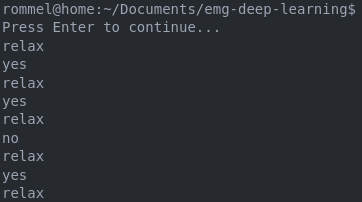
\includegraphics[width=0.65\linewidth]{images/annotations.png}}
    \\
  \subfloat[Connections to speech-focused muscle groups for EMG data.\label{Fig. 1b}]{%
        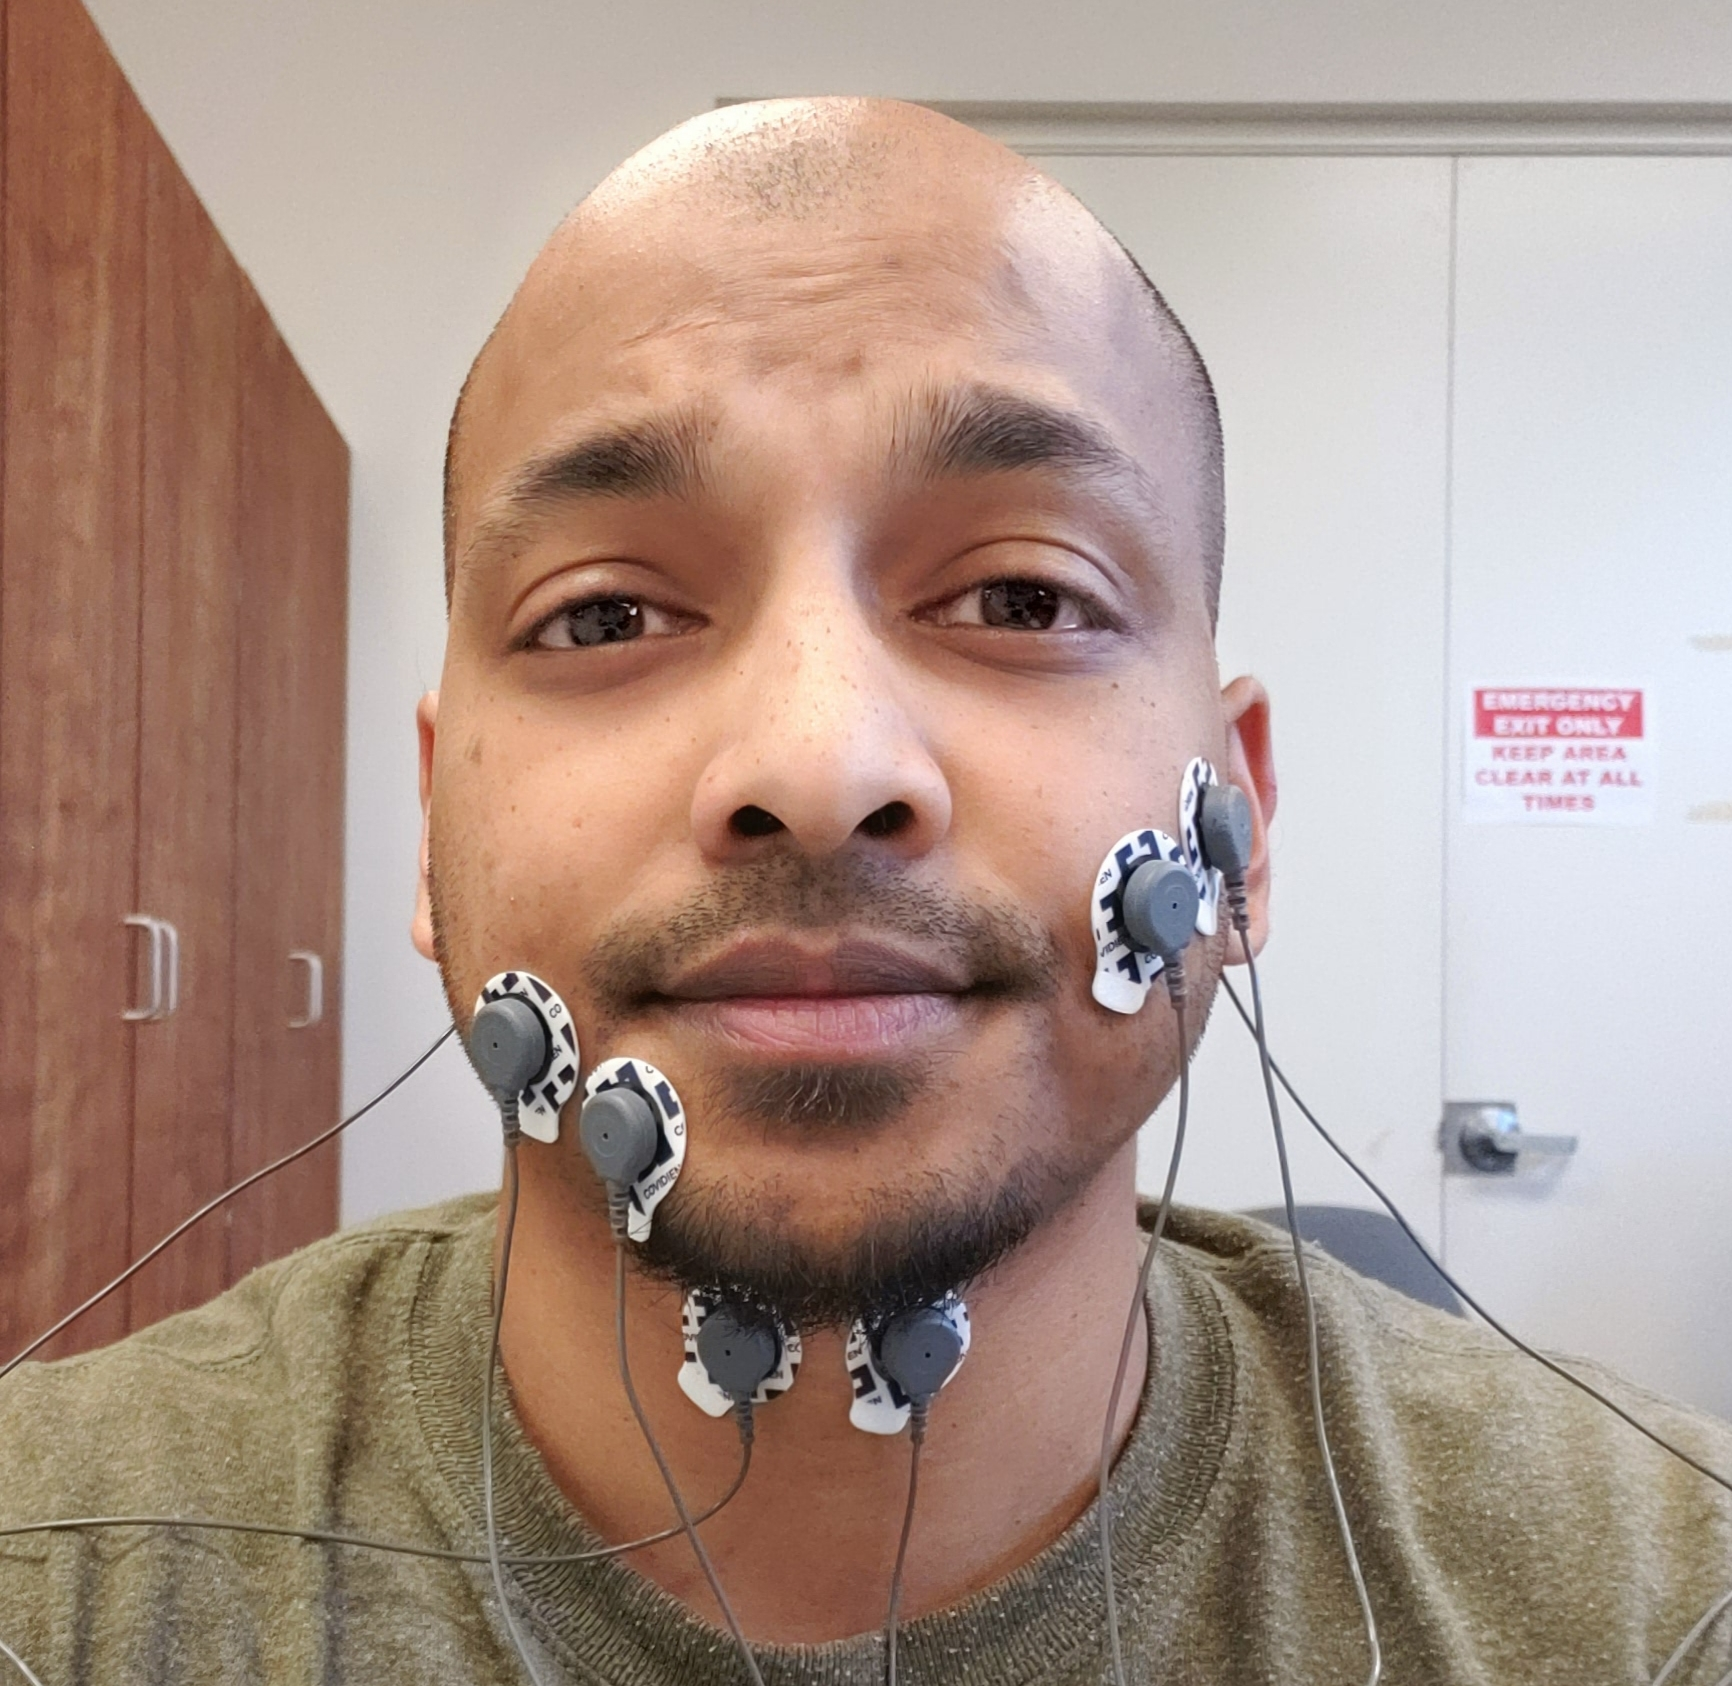
\includegraphics[width=0.65\linewidth]{images/face_leads.jpg}}
  \caption{Subjects reading rannotated labels on screen while connected to EMG units and electrodes.}
  \label{fig: conn-ann} 
\end{figure}

\subsubsection*{Cleaning Data}
Once the data is captured from the subjects, post processing of the data can begin. In order to remove the noise from the signals, filters are added after acquiring the data. We assumed that we are capturing muscle movements below 4 Hz. We also want to eliminate the 60 Hz interference from the surroundings. First, we applied a low-pass filter with a cutoff frequency of 4 Hz. The filters are designed around a window sinc function ~\cite{noauthor_how_nodate}. After applying a low pass filter, we add a high pass filter with a cutoff frequency of 0.5 Hz, which removes the associated DC offset. The coinciding timestamps of the EMG data with the annotations are mapped together to create an input-output relationship. \figurename \ref{fig: cleaned_signals} shows the filtered channels from the EMG with the respective annotated labels. This data will be used for the training and testing of the models. 

\begin{figure}[!t]
\centering
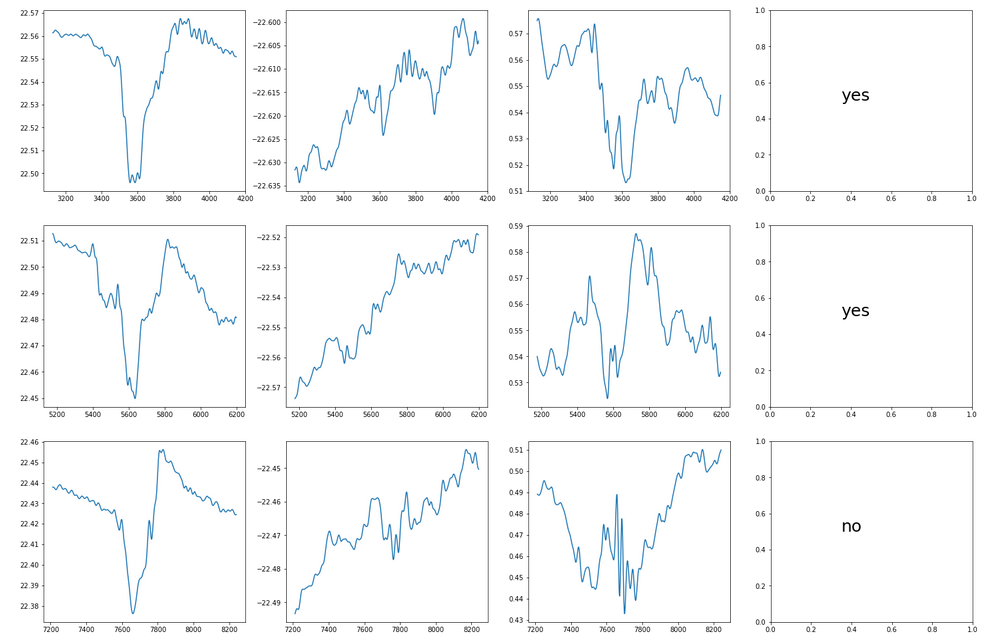
\includegraphics[width=3.5in]{images/cleaned_signals.png}
\caption{Signals after cleaning and adding low-pass and high-pass filters. First Column: EMG1, Second Column: EMG2, Third Column: EMG3, Fourth Column: Annotated Labels}
\label{fig: cleaned_signals}
\end{figure}

\section{Experimental Models}
\textit{Recurrent neural networks} (RNN), in particular LSTMs, are an effective tool for sequence processing that learn hidden representations of their sequential input. An LSTM can use its memory cells to remember long-range information and keep track of various attributes of data it is currently processing ~\cite{karpathy_visualizing_2016}. An LSTM, is built from an RNN, which works by unrolling data into N different copies of itself. Input of data from previous time steps $t_{n-1}$, $t_{n-2}$, $t_{n-3}$ \ldots, $t_{0}$ can be used when the current time-step $t_{n}$ is being evaluated. RNNs can learn temporal dependencies in the sequential data, and use it to classify new data. These unique capablities make RNNs and LSTMs ideal for classification of time-series data such as EMG signals. Adding multiple layers to LSTMs can improve results to experiments related to speech recognition, as investigated by ~\cite{graves_speech_2013}. In our experiment, we will use the sequential data from each EMG channel to classify the annotated labels in our data sets.

Another deep learning model that we investigated are \textit{Convolutional Neural Networks}. CNNs are made up of neurons that have learnable weights and biases. Each neuron receives an input and performs a series of matrix operations in order to predict classification scores ~\cite{noauthor_cs231n_nodate}. Most CNN architectures make the assumption that the inputs are images, which allow to encode values as matrices and perform dot product operations.  In order to convert sequential time-series data into image representations, we investigated \textit{Wavelet Transforms}, specifically Continuous Wavelet Transforms (CWT).

Unlike Fourier transform approaches that only show a signal representation in the frequency domain, wavelet transforms show both time and frequency representations. In ~\cite{janke_emg--speech:_2017}, ~\cite{kapur_alterego:_2018}, ~\cite{diener_session-independent_nodate}, they generated mel-frequency cepstral coefficients (MFCC), which creates one-dimensional representation that closely characterizes the envelopes of human speech to use as features in their respective models. In ~\cite{huzaifah_comparison_2017}, however states that time-frequency representations such as the CWT produced better accuracies than the MFCC features. The wavelet transform of a one-dimensional signal will generate coefficients as a two-dimension matrix of time-frequency representations, which is also known as a scaleogram. This scaleogram gives information about the dynamic behavior of the system, similar to that of a distinguishable image. Therefore, the wavelet transform represents a suitable method for the classification of EMG signals ~\cite{pauk_419._2008} by using CNN models ~\cite{huzaifah_comparison_2017}.

\section{Proposed Solution} \label{Proposed Solution}
Once the data is filtered and transformed, it will be ready for modeling. We used the two second window samples of when the subject repeated an annotated label on the screen, and dropped the instances where the word \textit{relax} existed. In our first experiment, we experimented with an LSTM model. The model is single direction LSTM, similar to ~\cite{janke_emg--speech:_2017},that consists of a LSTM layer with 100 filters followed by a Dense layer of 80 filters, and an output layer. The LSTM model is comprised of commonly used hyper-parameter values, such as a batch size of 32, with a learning rate of \textit{1e-4}. To measure the loss of the model, we used binary cross-entropy for the binary cases of \textit{yes} and \textit{no}, and categorical cross-entropy for the cases \textit{0-9}. We followed a many to one, sequence input architecture for the LSTM. The many to one architecture allows us to map many input sequences, in our case three, to a single output.

For our second experiment, we used a CNN architecutre as a deep learning model. We converted our singals into wavelet transforms, which generated scalograms that show resolution in the frequency and time-domains ~\cite{wletCNN}. Since there are three EMG channels of data, we created three sclaeograms per label, \figurename \ref{fig: wavelet_signals}. We then placed the three scaleograms on top of each other and created an image representation. The coefficients from the output of the scaleogram is then utilized as features to train the CNN model. The CNN architecture, similar to Lenet, is a two-layer model with a structure that can be represented as conv1-pool1-conv2-pool2-flat-dense-FC, with a  0.5 dropout before FC layer. The hidden convolutional layers have a size of 32, 64, and 512 filters respectively. The convolutional layers have a filter size of 3x3, and a max-pooling kernel size of 2x2, with a stride of 2. The hyper-parameters include a learning rate of \textit{1e-4} and batch size of 16. A smaller batch size is due to the fact of the large tensor size of the training data. Finally for the CWT parameters, we choose frequency bin size of 256 and a Mexican hat wavelet function. All of the models were trained on a Google Cloud Compute Engine with four virtual CPUs, 26 GB memory, and one NVIDIA Tesla K80 Graphics Processing Unit (GPU).

\begin{figure}[!tb]
\centering
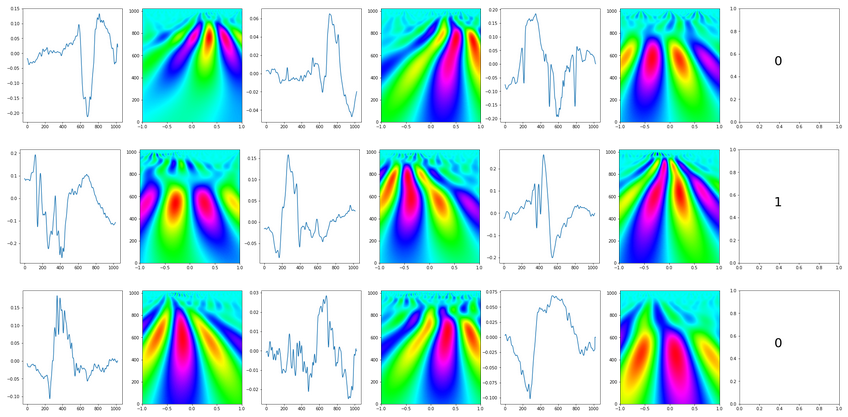
\includegraphics[width=3.5in]{images/wavelet_signal.png}
\caption{Continuous wavelet transform for each EMG channel as inputs, which maps to the labeled output.}
\label{fig: wavelet_signals}
\end{figure}


\section{Experimental Results}

To evaluate the performance of the deep learning models, we used precision and recall as identifying factors. In the experiments, recall is the fraction that the model actually predicted correct. Precision is the fraction of the model making a correct positive class classification.

\sisetup{table-format=2.2} 
\begin{table}[!h]
\centering
\caption{LSTM Model Results}
\begin{tabular}{|c|l|S|S|S|S|}           \hline 
\multirow{2}{*}{\# of class} &\multirow{2}{*}{type}    & \multicolumn{2}{c|}{Trained Data}    &\multicolumn{2}{c|}{Test Data}                    \\   \cline{3-6}
 &  &{Prec.} & {Rec.} & {Prec.}  & {Rec.}              \\   \hline 
\multirow{2}{*}{2} & no & 0.62 & 0.82 & 0.60  & 0.83   \\   \cline{2-6}  
 & yes & 0.72 & 0.47 & 0.77   & 0.52                \\   \hline
 \multicolumn{2}{|c|}{Average}   & 0.67 & 0.65 & 0.69 & 0.66 \\ \hline 
 \end{tabular}     
 %\caption{An important table}\label{Table. 1a}
 \label{Table 1: LSTM} 
\end{table}
 
\sisetup{table-format=2.2} 
\begin{table}[!h]
\centering
\caption{CWT-CNN Model Results }
\begin{tabular}{|c|l|S|S|S|S|}           \hline 
\multirow{2}{*}{\# of class} &\multirow{2}{*}{type}    & \multicolumn{2}{c|}{Trained Data}    &\multicolumn{2}{c|}{Test Data}                    \\   \cline{3-6}
 &  &{Prec.} & {Rec.} & {Prec.}  & {Rec.}              \\   \hline 
\multirow{2}{*}{2} & no & 0.97 & 0.95 & 0.75  & 0.72   \\   \cline{2-6}  
 & yes & 0.95 & 0.97 & 0.76   & 0.79                \\   \hline
 \multicolumn{2}{|c|}{Average}   & 0.96 & 0.96 & 0.76 & 0.76 \\ \hline 
 \end{tabular}     
 %\caption{An important table}\label{Table. 1a}
 \label{Table 2: CWT-CNN} 
\end{table}

Table \ref{Table 1: LSTM} shows the precision and recall for the LSTM model in our binary classification case. Table \ref{Table 2: CWT-CNN} shows the continuous wavelet transform with the CNN approach. The CWT-CNN model performs significantly better for both training and test data sets when compared to the LSTM model. On average for the binary test cases of \textit{yes} and \textit{no}, the CWT-CNN model had precision score of 82\%, and the LSTM model had a precision score of 61.5\%. For the multi-class test cases of \textit{0-9}, the results were not as favorable with an average precision score around 10\% for both LSTM and CWT-CNN models.

\section{Discussion}

In comparison with  ~\cite{janke_emg--speech:_2017}, ~\cite{kapur_alterego:_2018}, ~\cite{diener_session-independent_nodate}, who used similar deep learning models, thier results achieved better accuracy when compared to the work in this paper. A  contributing factor to their increase in performance is the amount of data they had available for thier training and testing purposes. In ~\cite{kapur_alterego:_2018}, approximately 31 hours of training data was captured in order to train their one-dimensional CNN model. In ~\cite{janke_emg--speech:_2017}, ~\cite{diener_session-independent_nodate}, who trained a variety of different models, utilized on-going corpus of data from previous research projects that focused on EMG-SSI systems. We have shown for a small data corpus, CNN based models perform better than LSTM models. With additional data, we believe that our models for binary and multi-class labels can be on par with other EMG-SSI systems using deep learning that were researched in this paper.

One of the ways our model differentiates and possibly improves is the use of CWT over MFCC. The MFCC requires windowed sampling in small increments. The output of the MFCC are one-dimensional coefficients, while CWT outputs coefficients in two-dimensions, allowing deep learning models such as CNN to learn and extract more features ~\cite{huzaifah_comparison_2017}. In previous research, MFCC were primary used for shallow learning speech recognition models such as HMM. As deep learning and CNN models continue to gain popularity, the use of mult-dimensional transformation techniques such as CWT will become more prevalent for speech recognition SSI systems. 

The transformation of data, specifically one-dimensional signals to its time-frequency components requires significant processing power. Resource limited systems cannot perform such laborious processes. We trained our models on a cloud computing engine which had the capability of increasing CPU and GPU power. These systems can become costly as the number of dedicated resources are assigned to the task of training a model. One has to justify the efforts of performance versus cost, specifically if the models improvements are only a few percentage. In terms of speech recognition, accuracy is important, the ability recognize speech patterns from a SSI system with high accuracy is a long-term goal.  

\section{Future Work}

One of the main ways to improve accuracy in our models is to acquire more training data. Getting subjects to volunteer can at times be challenging, more importantly annotating EMG data with proper labels. Acquiring more data would allow us to also train a variety of words and phrases, so that we can eventually build a robust SSI system. In our model, we eliminated instances where the subject was told to \textit{rest}. Future models should incorporate the \textit{rest} instances as an additional class, so that the model will learn to identify false positives.

The eventual goal is to build an SSI system that can improve its word recognition capablity over time as more data from similar SSI systems relay information over the network; resembling a Wireless Sensor Network and the Internet of Things ~\cite{ferdoush_wireless_2014}. A Bluetooth SSI system would communicate with a base station, process the data through the model, and output the results via an audio or visual interface. As more data is collected, deep learning models would be updated in the cloud, and pushed back to the base stations for processing. 
 
 
\section{Conclusion}

We have shown by using well-known deep learning methods we can effectively create models to recognize non-audible speech using surface EMG. This type of research is critical in designing SSI systems that can be used to interface with people who suffer from speech related problems. The experiments conducted by gathering data from a small sample of subjects showed that, CNN models tend to perform better than LSTM models, in terms of speed, accuracy, and precision in recognizing non-audible speech. Our approach of CWT with a combination of CNN also led to similar results when compared to previous research; however the cost of running such model may outweigh the benefits. In the future, finding ways to capture more robust data will be critical in training precise models that can disseminate and recognize a variety of words or phrases for SSI systems.
 
% An example of a floating figure using the graphicx package.
% Note that \label must occur AFTER (or within) \caption.
% For figures, \caption should occur after the \includegraphics.
% Note that IEEEtran v1.7 and later has special internal code that
% is designed to preserve the operation of \label within \caption
% even when the captionsoff option is in effect. However, because
% of issues like this, it may be the safest practice to put all your
% \label just after \caption rather than within \caption{}.
%
% Reminder: the "draftcls" or "draftclsnofoot", not "draft", class
% option should be used if it is desired that the figures are to be
% displayed while in draft mode.
%
%\begin{figure}[!th]
%\centering
%\includegraphics[width=2.5in]{myfigure.jpg}
%%where an .eps filename suffix will be assumed under latex,
%%and a .pdf suffix will be assumed for pdflatex; or what has been declared
%%via \DeclareGraphicsExtensions.
%\caption{Simulation Results.}
%\label{fig_sim}
%\end{figure}

% Note that IEEE typically puts floats only at the top, even when this
% results in a large percentage of a column being occupied by floats.

% Example of figure that shows 4x4 images 
%\section{A}
%\lipsum

%\section{B}
%\lipsum[1-3]
%\begin{figure} 
%    \centering
%  \subfloat[a\label{1a}]{%
%       \includegraphics[width=0.45\linewidth]{myfigure.jpg}}
%    \hfill
%  \subfloat[b\label{1b}]{%
%        \includegraphics[width=0.45\linewidth]{myfigure.jpg}}
%    \\
%  \subfloat[c\label{1c}]{%
%        \includegraphics[width=0.45\linewidth]{myfigure.jpg}}
%    \hfill
%  \subfloat[d\label{1d}]{%
%        \includegraphics[width=0.45\linewidth]{myfigure.jpg}}
%  \caption{test.}
%  \label{fig1} 
%\end{figure}
%\lipsum[1-5]


% An example of a double column floating figure using two subfigures.
% (The subfig.sty package must be loaded for this to work.)
% The subfigure \label commands are set within each subfloat command,
% and the \label for the overall figure must come after \caption.
% \hfil is used as a separator to get equal spacing.
% Watch out that the combined width of all the subfigures on a
% line do not exceed the text width or a line break will occur.
%
%\begin{figure*}[!h]
%\centering
%\subfloat[Case I]{\includegraphics[width=2.5in]{myfigure.jpg}
%\label{fig_first_case}}
%\hfil
%\subfloat[Case II]{\includegraphics[width=2.5in]{myfigure.jpg}
%\label{fig_second_case}}
%\caption{Simulation results.}
%\label{fig_sim}
%\end{figure*}
%
% Note that often IEEE papers with subfigures do not employ subfigure
% captions (using the optional argument to \subfloat[]), but instead will
% reference/describe all of them (a), (b), etc., within the main caption.


% An example of a floating table. Note that, for IEEE style tables, the
% \caption command should come BEFORE the table. Table text will default to
% \footnotesize as IEEE normally uses this smaller font for tables.
% The \label must come after \caption as always.
%
%\begin{table}[!t]
%%% increase table row spacing, adjust to taste
%\renewcommand{\arraystretch}{1.3}
%% if using array.sty, it might be a good idea to tweak the value of
%% \extrarowheight as needed to properly center the text within the cells
%\caption{An Example of a Table}
%\label{table_example}
%\centering
%%% Some packages, such as MDW tools, offer better commands for making tables
%%% than the plain LaTeX2e tabular which is used here.
%\begin{tabular}{|c||c|}
%\hline
%One & Two\\
%\hline
%Three & Four\\
%\hline
%\end{tabular}
%\end{table}


% Note that IEEE does not put floats in the very first column - or typically
% anywhere on the first page for that matter. Also, in-text middle ("here")
% positioning is not used. Most IEEE journals/conferences use top floats
% exclusively. Note that, LaTeX2e, unlike IEEE journals/conferences, places
% footnotes above bottom floats. This can be corrected via the \fnbelowfloat
% command of the stfloats package.



%\section{Conclusion}
%The conclusion goes here.


% conference papers do not normally have an appendix


% use section* for acknowledgement
%\section*{Acknowledgment}


%The authors would like to thank.....





% trigger a \newpage just before the given reference
% number - used to balance the columns on the last page
% adjust value as needed - may need to be readjusted if
% the document is modified later
%\IEEEtriggeratref{8}
% The "triggered" command can be changed if desired:
%\IEEEtriggercmd{\enlargethispage{-5in}}

% references section

% can use a bibliography generated by BibTeX as a .bbl file
% BibTeX documentation can be easily obtained at:
% http://www.ctan.org/tex-archive/biblio/bibtex/contrib/doc/
% The IEEEtran BibTeX style support page is at:
% http://www.michaelshell.org/tex/ieeetran/bibtex/
\bibliographystyle{IEEEtran}
% argument is your BibTeX string definitions and bibliography database(s)
\bibliography{first_draft}
%
% <OR> manually copy in the resultant .bbl file
% set second argument of \begin to the number of references
% (used to reserve space for the reference number labels box)
%\begin{thebibliography}{1}
%
%\bibitem{IEEEhowto:kopka}
%H.~Kopka and P.~W. Daly, \emph{A Guide to \LaTeX}, 3rd~ed.\hskip 1em plus
%  0.5em minus 0.4em\relax Harlow, England: Addison-Wesley, 1999.
%
%\end{thebibliography}

% that's all folks
\end{document}
